%%% LaTeX Template: Newsletter
%%%
%%% Source: http://www.howtotex.com/
%%% Feel free to distribute this template, but please keep the referal to HowToTeX.com.
%%% Date: September 2011


%%% ---------------
%%% PREAMBLE
%%% ---------------
\documentclass[10pt,a4paper]{article}

% Define geometry (without using the geometry package)
\setlength\topmargin{-48pt}
\setlength\headheight{0pt}
\setlength\headsep{25pt}
\setlength\marginparwidth{-20pt}
\setlength\textwidth{7.0in}
\setlength\textheight{9.5in}
\setlength\oddsidemargin{-30pt}
\setlength\evensidemargin{-30pt}

\frenchspacing						% better looking spacing

% Call packages we'll need
\usepackage[utf8]{inputenc}
\usepackage{CJKutf8}
\newenvironment{Japanese}{%
  \CJKfamily{min}%
  \CJKtilde
  \CJKnospace}{}
\usepackage[english,ukrainian]{babel}			% languages
\usepackage{graphicx}				% images
\usepackage{amssymb,amsmath}		% math
\usepackage{multicol}				% three-column layout
\usepackage{url}					% clickable links
\usepackage{marvosym}				% symbols
\usepackage{wrapfig}				% wrapping text around figures
\usepackage[T1,T2A]{fontenc}			% font encoding
\usepackage{charter} 				% Charter font for main content
\usepackage{blindtext}				% dummy text
\usepackage{datetime}				% custom date
	\newdateformat{mydate}{\monthname[\THEMONTH] \THEYEAR}
\usepackage[pdfpagemode=FullScreen,
			colorlinks=false]{hyperref}	% links and pdf behaviour

\makeatletter\chardef\l@japanese=255 \makeatother

% Customize (header and) footer
\usepackage{fancyhdr}
\pagestyle{fancy}
\lfoot{	\footnotesize 
Спільнота українців Японії ''Краяни'' / 
\begin{CJK}{UTF8}{}
\begin{Japanese}
在日ウクライナ人コミュニティ「クラヤニイ」
\end{Japanese}
\end{CJK}
\\
		\Mundus\ \href{https://www.facebook.com/ukrainians.japan}{www.facebook.com/ukrainians.japan}	\quad
	  }
\cfoot{}
\rfoot{\footnotesize ~\\ Сторінка \thepage}
\renewcommand{\headrulewidth}{0.0pt}	% no bar on top of page
\renewcommand{\footrulewidth}{0.4pt}	% bar on bottom of page

%%% ---------------
%%% DEFINITIONS
%%% ---------------

% Define separators
\newcommand{\HorRule}[1]{\noindent\rule{\linewidth}{#1}} % Creating a horizontal rule
\newcommand{\SepRule}{\noindent							 % Creating a separator
						\begin{center}
							\rule{250pt}{1pt}
						\end{center}
						}						

% Define Title en News input
\newcommand{\JournalName}[1]{%
		\begin{center}	
			\Huge \usefont{T2A}{augie}{m}{n}
			#1%
		\end{center}	
		\par \normalsize \normalfont}
		
\newcommand{\JournalIssue}[1]{%
		\hfill \textsc{\mydate \today, Випуск №1}
		\par \normalsize \normalfont}

\newcommand{\NewsItem}[1]{%
		\usefont{T2A}{iwona}{m}{n} 
		\large #1 \vspace{4pt}
		\par \normalsize \normalfont}
		
\newcommand{\NewsAuthor}[1]{%
			\hfill \textsc{#1} \vspace{4pt}
			\par \normalfont}		


%%% ---------------
%%% BEGIN DOCUMENT
%%% ---------------
\begin{document}
% Title	
% -----
\JournalIssue{1}
\JournalName{Краяни - часопис українців Японії}
\noindent\HorRule{3pt} \\[-0.75\baselineskip]
\HorRule{1pt}
% -----

% Front article
% -----
\vspace{0.5cm}
	\SepRule
\vspace{0.1cm}

\begin{center}
\begin{minipage}[h]{0.75\linewidth}
	\begin{wrapfigure}{l}{0.61\textwidth}
		\includegraphics[width=0.62\textwidth]{images/bunkamura}
		\\	% this spacer is needed to make the text on the right fit OK
	\end{wrapfigure}
	\NewsItem{Писанки в Шібуя}
Виставка робіт українських та японських майстринь писанкарства була представлена на щорічній виставці ''Bunkamura Craft Collection 2015'', що в районі Шібуя Токіо.
\vspace{3.3cm}
\end{minipage}
\end{center}
% -----

% Page 1
\vspace{0.5cm}
	\SepRule
\vspace{0.5cm}
\begin{multicols}{3}
	\NewsItem{Вітаємо з перемогою!}
	\NewsAuthor{Москва}
		\begin{center}
			\includegraphics[width=0.8\linewidth]{images/rapiry}
		\end{center}
Вітаємо Олега Мацейчука - українця, головного тренера з фехтування на рапірах Японії, з перемогою вихованця, чемпіона світу з фехтування Юкі Ота (Японія). 
У фіналі чемпіонату світу серед чоловіків у двобої з американцем переміг японець. Золото з фехтування на рапірах стало першим в історії Японії.
Олег Мацейчук - киянин, екс-фехтувальник збірної України. В 2003 розпочав роботу тренером з фехтування в Японії. За період перебування в Японії виховав ціле покоління спортсменів, які вже самі стали тренерами.
Успіхів та нових досягнень!
% -----

\vspace{1cm}
% -----
\NewsItem{Цікаві семінари в Кансай}
\NewsAuthor{Кіото}
		\begin{center}
			\includegraphics[width=0.8\linewidth]{images/seminary}
		\end{center}
Запрошуємо усіх, хто цікавиться українською культурою, відвідати ''Цікаві семінари'', що організує спільнота українців у Кансаї. На семінарах ми розкажемо про основні поточні події у житті спільноти, познайомимо з історією, мистецтвом і культурою нашої країни. Семінари відбудуться 11-го і 25-го липня (субота) з 15:00 до 16:30 у кокока (Міжнародному Центрі міста Кіото). Участь у семінарах платна: 1,000 ієн за участь у 2-х семінарах. Кошти від семінару підуть на розвиток української громади. Також будемо збирати пожертви для постраждалих у війні на сході. Ми готуємо багато цікавих презентацій. Учасники семінарів зможуть вдягнути український костюм, а також скуштувати українських солодощів. Семінари будуть проходити японською мовою. 
\end{multicols}

% Page 2
\begin{multicols}{3}

	\NewsItem{Благодійний концерт}
	\NewsAuthor{Йокогама}
		\begin{center}
			\includegraphics[width=0.8\linewidth]{images/concert}
		\end{center}
20 червня в м. Йокогама відбувся благодійний концерт на підтримку Військового Госпіталю України ''Charity For Ukraine, 2015''.
Чудовий концерт організували талановиті артисти та виконавці різних країн: Elina-star, Kateryna, Yuliya, Viktoria, Amauri Marina, Cesar Canisales, Lana, Itsuki, Erina, Emma, Eshe, Anzy, Hikari, Leila, Yasmin. Захід відбувся за підтримки Посольства України в Японії.
% -----

\vspace{1cm}
% -----
\NewsItem{''Івасик Телесик'' в Японії}
\NewsAuthor{Токіо, школа ''Джерельце''}
		\begin{center}
			\includegraphics[width=0.8\linewidth]{images/telesyk}
		\end{center}
''Івасик Телесик'' в Токio на останньому уроці недільної школи Джерельце 14 червня. В День ''останнього дзвоника'' японського Джерельця вихованці школи порадували батьків та вчителів виставою, за казкою ''Івасик Телесик''. За успіхи у навчанні учні отримали вітальні грамоти та подарунки. Українська дитяча школа ''Джерельце'' була заснована у березні 2009 року в місті Токіо. Заняття в школі проводяться двічі на місяць кваліфікованими вчителями за власно розробленою програмою. Сьогодні кількість вихованців нараховує більше 40 учнів різних вікових категорій. Дітлахи мають змогу навчитись читанню, письму, математиці та мистецтву. Діти знайомляться з традиційними святами, готують Новорічні та Великодні вистави, Різдвяні Вертепи. Отримати більше інформації та записатись на заняття можна на сайті школи dzherelce.github.io 

\vspace{1cm}
	\NewsItem{3-й щорічний Мегамарш у вишиванках}
	\NewsAuthor{Токіо, Ґінза}
		\begin{center}
			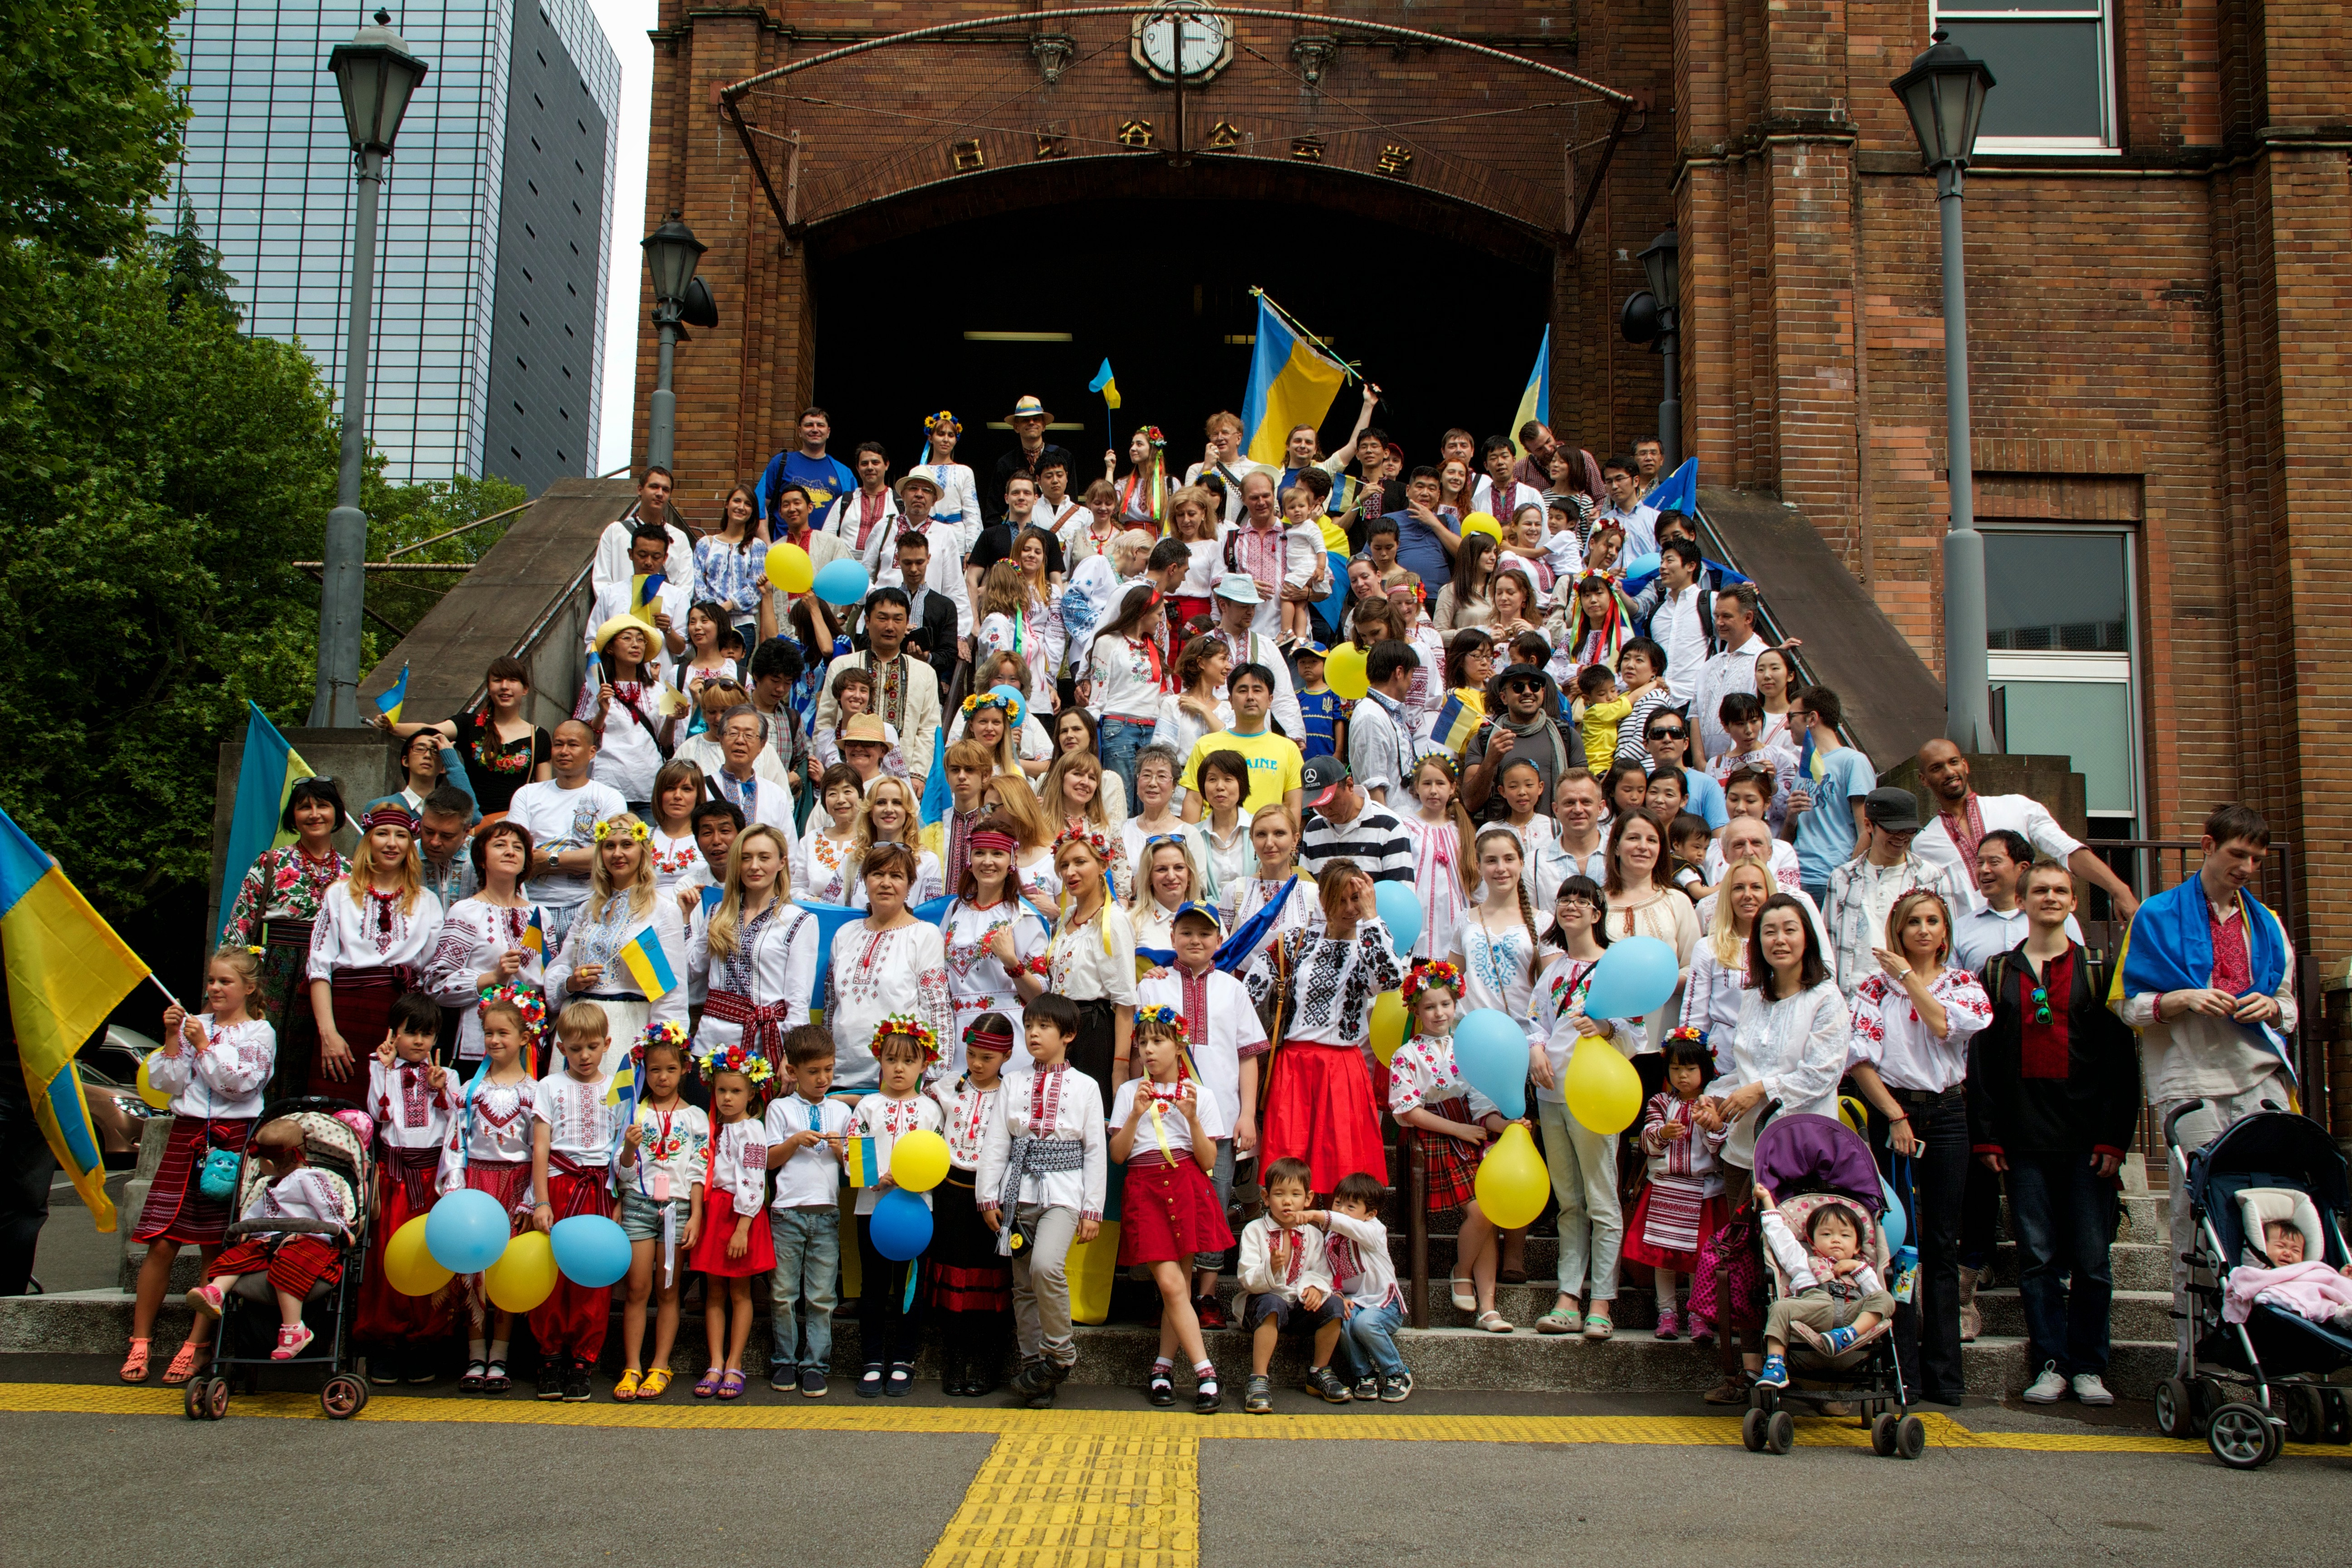
\includegraphics[width=0.8\linewidth]{images/megamarsh}
		\end{center}
Дякуємо всім, хто взяв участь у 3-му щорічному Мегамарші у вишиванках у Токіо! Більше 150 українців, японців та представників інших країн світу вийшли у вишитих сорочках та з прапорами України, викликавши неабиякий інтерес у місцевого населення. Захід був організований за підтримки Посольства України в Японії та місії Української Православної Церкви Київського Патріархату ''St. Jude Ukrainian Orthodox Mission'' в місті Токіо. Цьогорічний парад був присвячений співпраці між Україною та Японією. Прапор України, що побував на Майдані у Києві, до Токіо привезла студентка з Калуша, об'єднавши українців Японії з Батьківщиною. Захід підтримав дипломатичний сектор Посольства України в Японії і надзвичайний і повноважний Посол Ігор Харченко з сім'єю. У вишиванках приєднались екс-посол Японії в Україні Саката Тоїчі з дружиною, а також відомий українознавець та генерал-полковник Українського Реєстрового Козацтва Йошіхіко Окабе. Вишиванкова хода в Токіо стала гарною традицією, а постійно зростаюча чисельність учасників та активний інтерес японців до заходу підтвердили необхідність гуртування та створення українського осередку в Японії. Слава Україні!
% -----

\vspace{1cm}
% -----
\NewsItem{Токійський ''Козак''}
\NewsAuthor{Токіо}
		\begin{center}
			\includegraphics[width=0.8\linewidth]{images/kozak}
		\end{center}
Обирай українське, де б ти не був! Японці вражають своєю любов'ю до України та українського. Їдучи у справах по дорозі в Токіо українка почула сигнал іншого авто. Спочатку подумала, що вона порушила правила і за це їй сигналять. Її обганяє японець і з щасливою японською посмішкою вказує на свою машину, де наклейки з написом ''Україна'' та ''Козак'' та на її, де зображений український прапор. Так знаходять нових друзів по авто. Користуйтесь транспортними послугами ''Козака''! 

\end{multicols}

% -----
\end{document} 

